%preamble
\documentclass[letterpaper]{article}
\synctex=1
\usepackage{graphicx}
%\graphicspath{{images/}}

\usepackage{lipsum}
\usepackage{float}

\usepackage{amssymb}
\usepackage{amsmath}

\usepackage{siunitx}

\usepackage{multirow}
% for merging table cells I think

\usepackage{tabularx}
\renewcommand\tabularxcolumn[1]{m{#1}}% for vertical centering text in X column

% allows for linewrap within cells
\newcolumntype{Y}{>{\centering\arraybackslash}X}

\usepackage{todonotes}
\usepackage{hyperref}

\usepackage{pdfpages} % for attaching the table lol

\usepackage[section]{placeins} % forces figures to appear in the same section

%for plots
\usepackage{tikz}
\usepackage{pgfplots}
\pgfplotsset{width=8cm,compat=1.15}\usepgfplotslibrary{patchplots}
\title{ECE 322 \\
Lab Report 1}
\author{Arun Woosaree\\
XXXXXXX}
\begin{document}
\maketitle
\section{Introduction} The purpose of this lab was to serve as a practical
introduction to some more black box testing techniques. In this lab, the
testing methods introduced were the Extreme Point Combination (EPC), and the
Weak n x 1 strategy methods. We tested two programs written in Java using both
of these testing strategies. The first application, named Drone takes in three
arguments, and outputs either `Success!', `Failure', or an error message based
on whether the arguments are integers $\geq 0$, and their sum is less than
$k=100$. The second program, named RemoteCar takes in two arguments which
represent points on a Cartesian plane, and outputs either `Ok', `Out of range',
or an error message based on whether the point is on a circle of radius 1 about
the origin. The idea for EPC testing is to identify the input domain limits,
and produce all possible combinations of inputs with each of the input
variables taking on a minimum value, slightly under minimum, a maximum value,
and slightly over maximum value. One additional test case is added somewhere
within the valid subdomain to generate a total of $4^n + 1$ test cases, where
n is the dimension of inputs, or put more simply, the number of input
variables. With the weak n x 1 strategy, we attempt to find linear boundaries 
of the problem using domain analysis. $n$ points are selected on each linear
boundary, where $n$ is the number of input variables, and one additional point 
is chosen outside of each boundary. An additional point within the boundary is
chosen if the boundary is open, and if the boundary is instead closed an 
additional point outside the boundary is chosen. In the end, with the weak
n x 1 strategy, $b \times (n + 1)$ test cases are generated, where b is the 
number of linear boundaries, and n is the dimensionality, or the number of
inputs.

\section{Task 1 - Drone}
For task one in this lab, the Drone application was tested using both the
EPC method and the weak n x 1 strategy. Drone is a command-line program
written in java, which takes three inputs, $x_1$, $x_2$, and $x_3$.
If $x_1 + x_2 + x_3 \leq k$, where $k=100$, the program should output
`Success', and if not, it should output `Failure'. The three inputs 
must be integers $\geq 0$. 

\subsection{Sudomain Plot}
The subdomain for this problem is illustrated in the 3-Dimensional graph below:
\begin{figure}[H]
	\centering
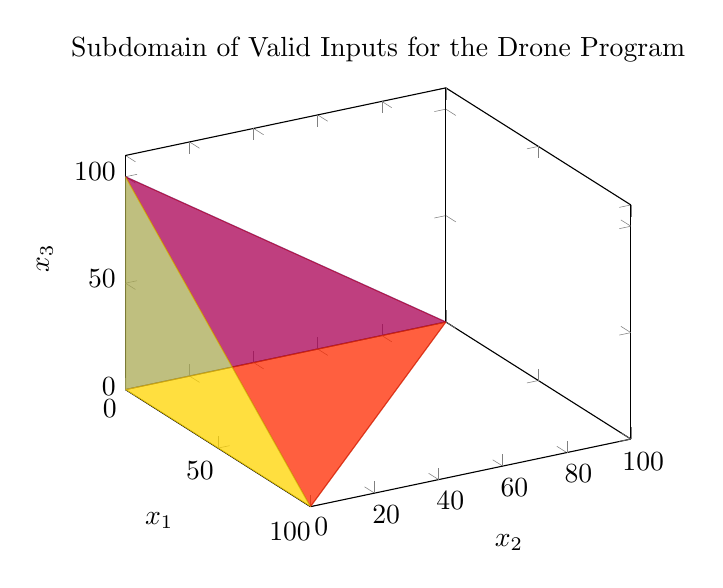
\begin{tikzpicture}
	\begin{axis}[view/h=60,xlabel=$x_1$,ylabel=$x_2$,zlabel=$x_3$,title={Subdomain of Valid Inputs for the Drone Program},zmin=0]
\addplot3 [
opacity=0.5,
table/row sep=\\,
patch,
patch type=polygon,
vertex count=3,
patch table with point meta={
% pt1 pt2 pt3 pt4 pt5 cdata
0 1 2 0\\
0 1 3 1\\
0 2 3 2\\
1 2 3 3\\
},
] table {
x y z\\
0 0 0 \\%0
0 0 100\\%1
0 100 0\\%2
100 0 0\\%3
};
\end{axis}
\end{tikzpicture}
\caption{Valid inputs for the Drone program. $x_1 + x_2 + x_3 \leq 100\ |\ x_1, x_2, x_3 \geq 0$}
\end{figure}

\subsection{EPC Strategy}
Using the EPC strategy, since there are 3 input variables, there are
$4^3 + 1 = 65$ test cases. The values chosen were:
\begin{itemize}
	\item max: 100
	\item min: 0
	\item slightly under min: -1
	\item slightly over max: 101
\end{itemize}
All the permutations of the 3 inputs taking on these values were generated
and tested. An additional test case was created within the valid subdomain,
which was $(x_1, x_2, x_3) = (10, 20, 30)$. The full table of test cases
along with their expected inputs and outputs can be found in Appendix A of this
report. The failed test cases are highlighted in red for convenience.

\subsection{Weak n x 1 Strategy}
Using the weak n x 1 strategy, there are 4 boundary surfaces to take into
consideration. Since there are 3 inputs, we pick 3 points on each boundary
surface, and one additional point outside of each boundary, for a total of
$4\times (3 + 1) + 1 = 17$ test cases. The additional test case chosen inside
the boundary was $(x_1, x_2, x_3) = (30, 20, 10)$. The table of test cases
along with their expected inputs and outputs can be found in Appendix B of this
report. The failed test cases are highlighted in red for convenience.

\subsection{Discussion}
Using both the EPC and the weak n x 1 strategy, we see that for all of the
failed test cases, the input variable $x_2$ is a negative. For negative
inputs, the program is expected to give an error telling the user that 
negative inputs are not valid. Instead, the program outputs `Success!'
or `Failure!' when $x_2 < 0$. Using the EPC strategy, we see
2 types or failures, where the program outputs both `Success!'                       
or `Failure!'; however, with the weak n x 1 strategy we only saw the case where
`Success!' is outputted mistakenly. It should be noted however, that both
testing strategies found an error which seems to stem from the same issue,
(the application not checking if $x_2$ is negative, and the weak n x 1 strategy
did so with less test cases (17 versus 65). As a result, for this problem,
the weak n x 1 strategy seemed to be both more efficient and effective,
since the same problem was caught using the EPC strategy but with far fewer
test cases.


\section{Part 2 - RemoteCar}
For task two in this lab, the RemoteCar application was tested using both the
EPC method and the weak n x 1 strategy. RemoteCar is a command-line program
written in Java, which takes two inputs, $x$, and $y$, which represent a
point on the Cartesian plane.
If $(x,y)$ falls on the circle with radius $r=1$, centered about the origin,
the program will output`Ok.', or `Out of range!'. The input arguments must
be real numbers, or the program should output an error letting the user know
that the argument entered was not a number.

\subsection{Subdomain Plot}
Since circular boundaries are too complex to test using linear methods,
we approximate the circular subdomain with $m$ linear segments. In this lab,
we carried out the testing with $m=4$ linear boundaries to test a circular
boundary of radius 1 about the origin. The accuracy of the approximation
could have been increased by increasing the number of linear boundaries.
For example, $m=8$ which would make an octagon shape would be a more accurate
representation of the circle, and as $m \to \infty$ we would get closer
and closer to the actual boundary.

\begin{figure}[h]
	\centering
	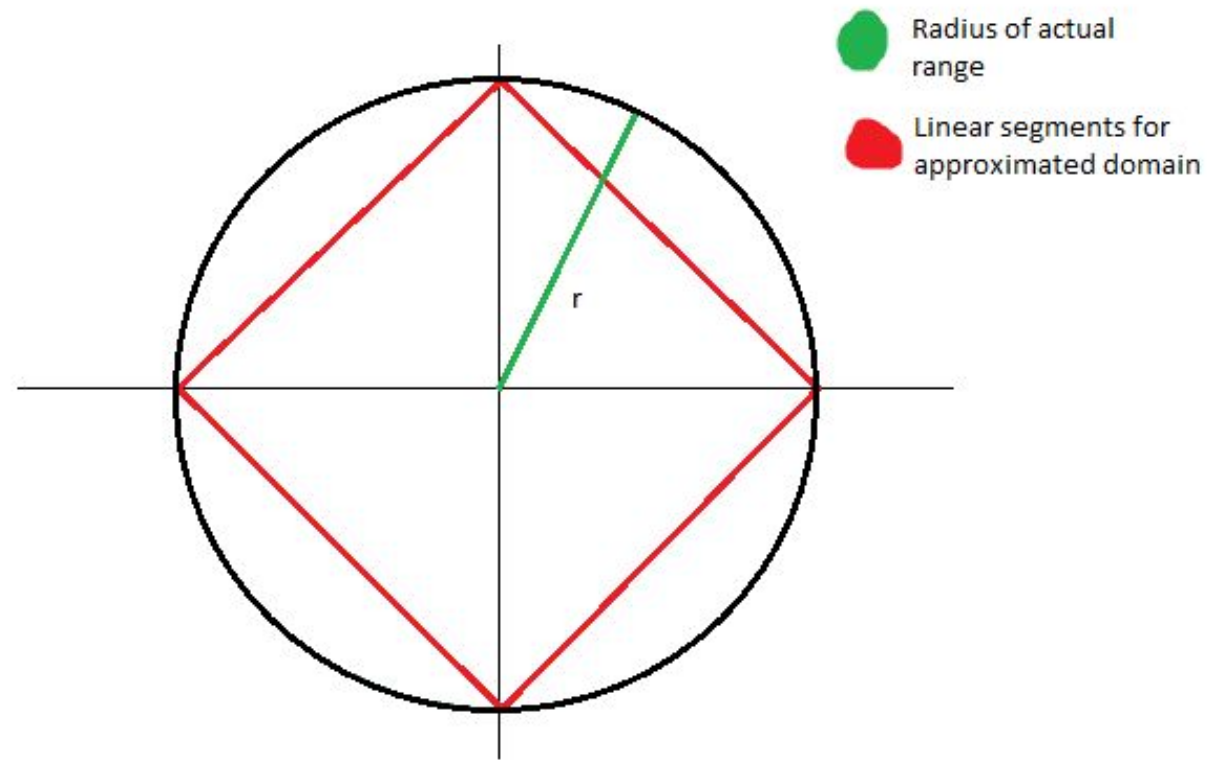
\includegraphics{remotecar-subdomain.png}
	\caption{Approximate subdomain $m=4$ shown in red.
		Circle is centered at the origin, $r=1$.
	        Plot taken from the lab instructions.}
\end{figure}

The equations of the approximated linear boundaries are as follows:
	\[ y= \begin{cases} 
      1-x &  0 \leq x \leq 1 \\
      1+x &  -1 \leq x \leq 0 \\
      -(1+x) &  -1 \leq x \leq 0 \\
      x-1 &  0 \leq x \leq 1 \\
   \end{cases}
\]
\FloatBarrier

\subsection{EPC Strategy}
Using the EPC strategy, since there are 2 input variables, there are
$4^2 + 1 = 17$ test cases. The values chosen were:
\begin{itemize}
	\item max: 1
	\item min: -1
	\item slightly under min: -1.1
	\item slightly over max: 1.1
\end{itemize}
All the permutations of the 2 inputs taking on these values were generated
and tested. An additional test case was created within the valid subdomain,
which was $(x,y) = (0, 0)$. The full table of test cases
along with their expected inputs and outputs can be found in Appendix C of this
report. Failed test cases would have been highlighted in red, however,
there were no test faliures were found using this strategy.

\subsection{Weak n x 1 Strategy}
Using the weak n x 1 strategy, there are 4 boundary lines to take into
consideration. Since there are 2 inputs, we pick 2 points on each boundary
line, and one additional point outside of each boundary, for a total of
$4\times (2 + 1) + 1 = 13$ test cases. The additional test case chosen inside
the boundary was $(x, y) = (0.3, 0.7)$. The table of test cases
along with their expected inputs and outputs can be found in Appendix D of this
report. The failed test cases are highlighted in red for convenience.

\subsection{Discussion}
The domain approximation is somewhat effective. It seems to work best if
test inputs chosen are far away from the boundaries, since there is a risk
of a false negative test result if the chosen test input is too close to the
boundary. This can happen when the test case chosen is outside of the
approximated boundary, while it is still in the actual subdomain's boundary.
In such a scenario, we might expect a test case to fail using the
approximation, yet if the program is running correctly, the test case will
pass. The configuration could have been adjusted to yield higher accuracy
of the subdomain. For example, we could have increased the number of linear
boundaries. Using the EPC strategy, the complexity of testing is unaltered. 
There are still 17 test cases, and they would all be the same. However,
using the weak n x 1 strategy, the complexity would be increased.
We would have to make $b \times (2 + 1) + 1$ test cases, where b is
the number of linear boundaries we choose to use for the approximation.
In other words, we would need an additional 3 test cases for each boundary
we add to increase the accuracy. 

For this problem, it seems that the EPC testing strategy is more accurate.
Using the weak n x 1 strategy, we ran into some cases where the test input
was outside of our approximated boundary, yet it was inside the actual
subdomain. This resulted in 4 test case failures, which were not actual
errors with the program itself, but rather due to the innacurate linear
approximation of the subdomain. As a result, no actual errors were identified 
in the application. In this case, with $m=4$ boundaries, the number of test
cases for the EPC and weak n x 1 strategies were similar. However, 
the weak n x 1 strategy could have a lot more test cases if we added more 
linear boundaries to make a better approximation of the problem's subdomain.

\section{Conclusion}
In this lab, we were introduced to black-box testing. The techniques
learned were dirty testing, error guessing, and partition-based testing.
Dirty testing's strength seems to also be its weakness at the same time. That is,
the test cases written are only limited by the tester's creativity.
One disadvantage, however, is that one can generate a lot of extra test cases
that are arguably unnecessary. That is, there is the possibility of having multiple
tests which cover the same functionality of the program. This is a problem that
using the partition-based testing method addressed. While equivalence testing allowed us 
to write significantly fewer test cases,
it does not catch some unique cases. For example, if dirty testing was done instead,
one might have tried the test inputs $$1111111111\ 1111111111\ 1$$, which returns ERROR: Invalid triangle
instead of saying that it's an isosceles one. This error, and potentially others were not
caught using partition-based testing. What is interesting, though is that the one
test failure with inputs (2 2 4) for the Triangle program allowed for another error to be found, which is
the case where an input like (1 2 3) which should cause an error instead returns `Scalene'.
Overall, it would not be fair to say that
one testing method is universally better than the other, however, the tester would
need to use their judgement and experience to choose an appropriate testing method
for the software that they want to test.

\vfill
\appendix
%\section*{Appendix}

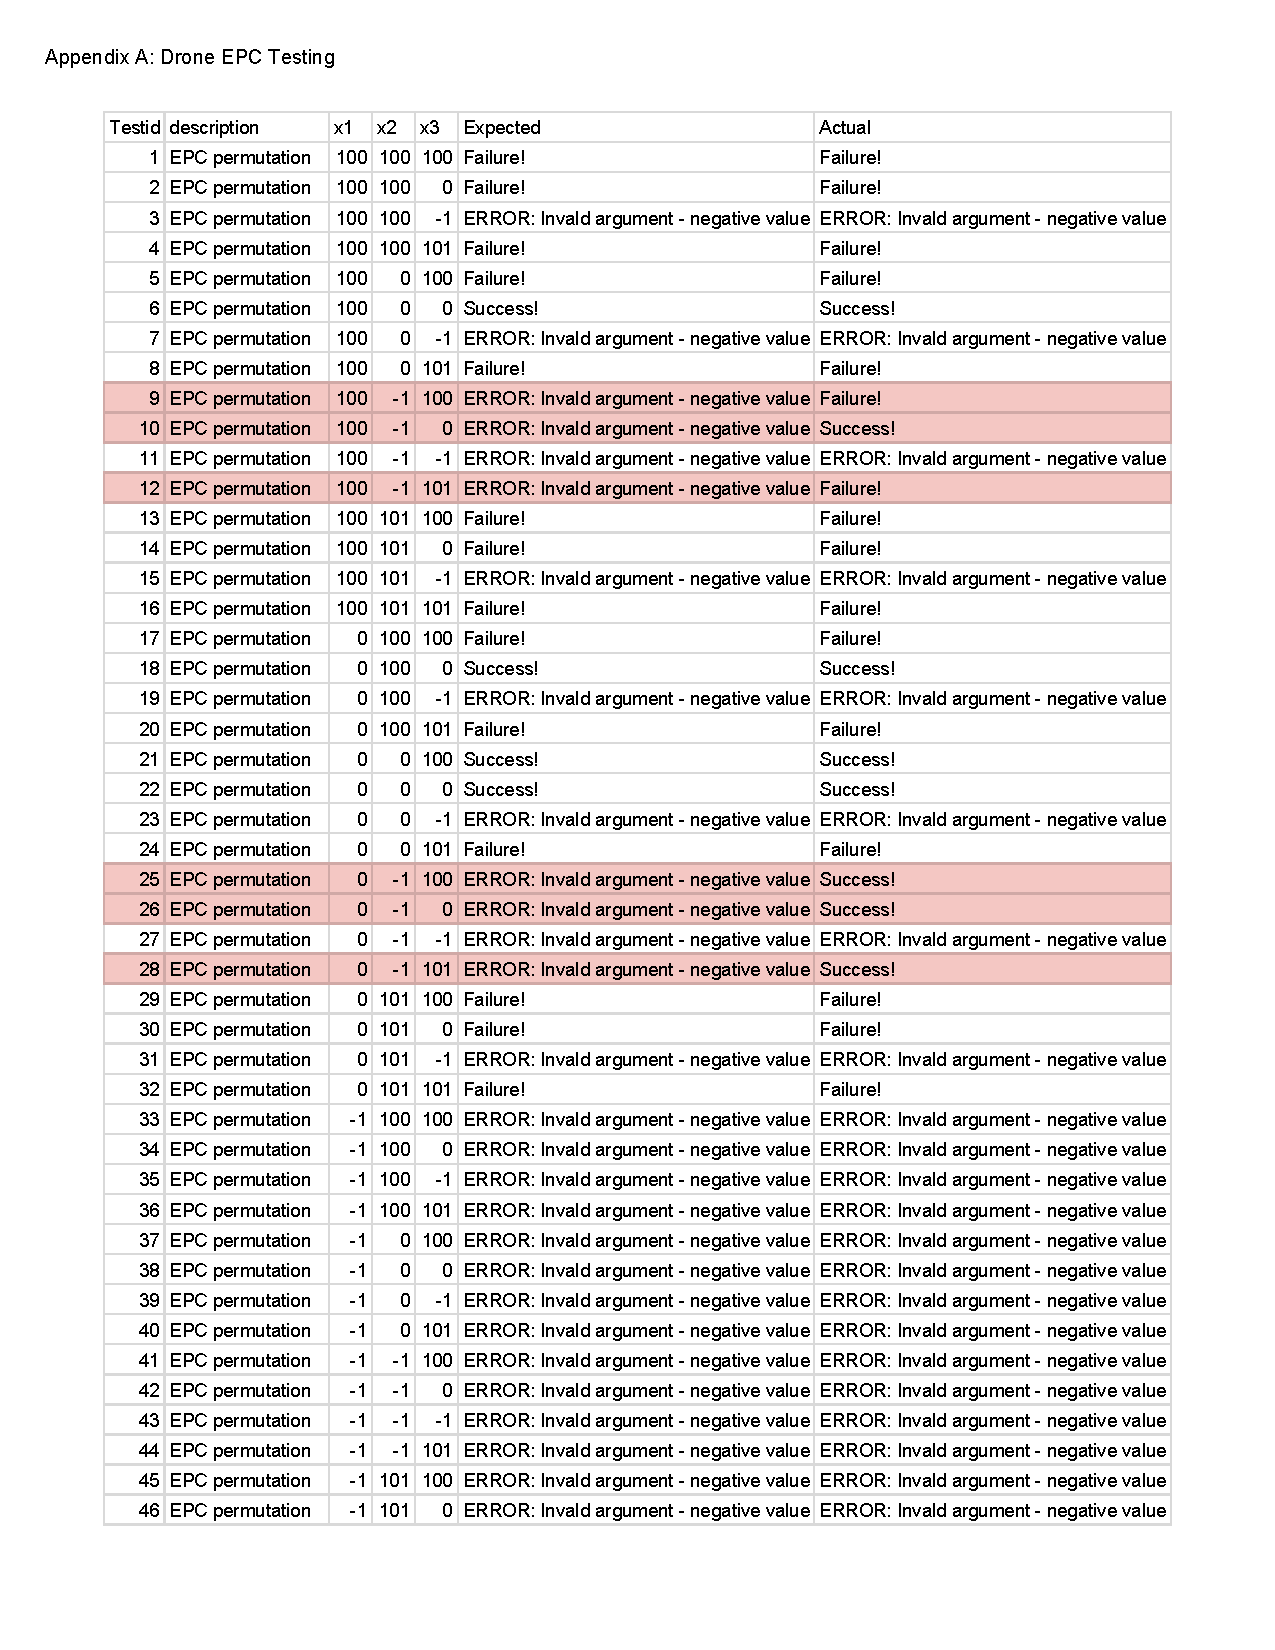
\includepdf[pages=-]{EPC-drone-table.pdf}
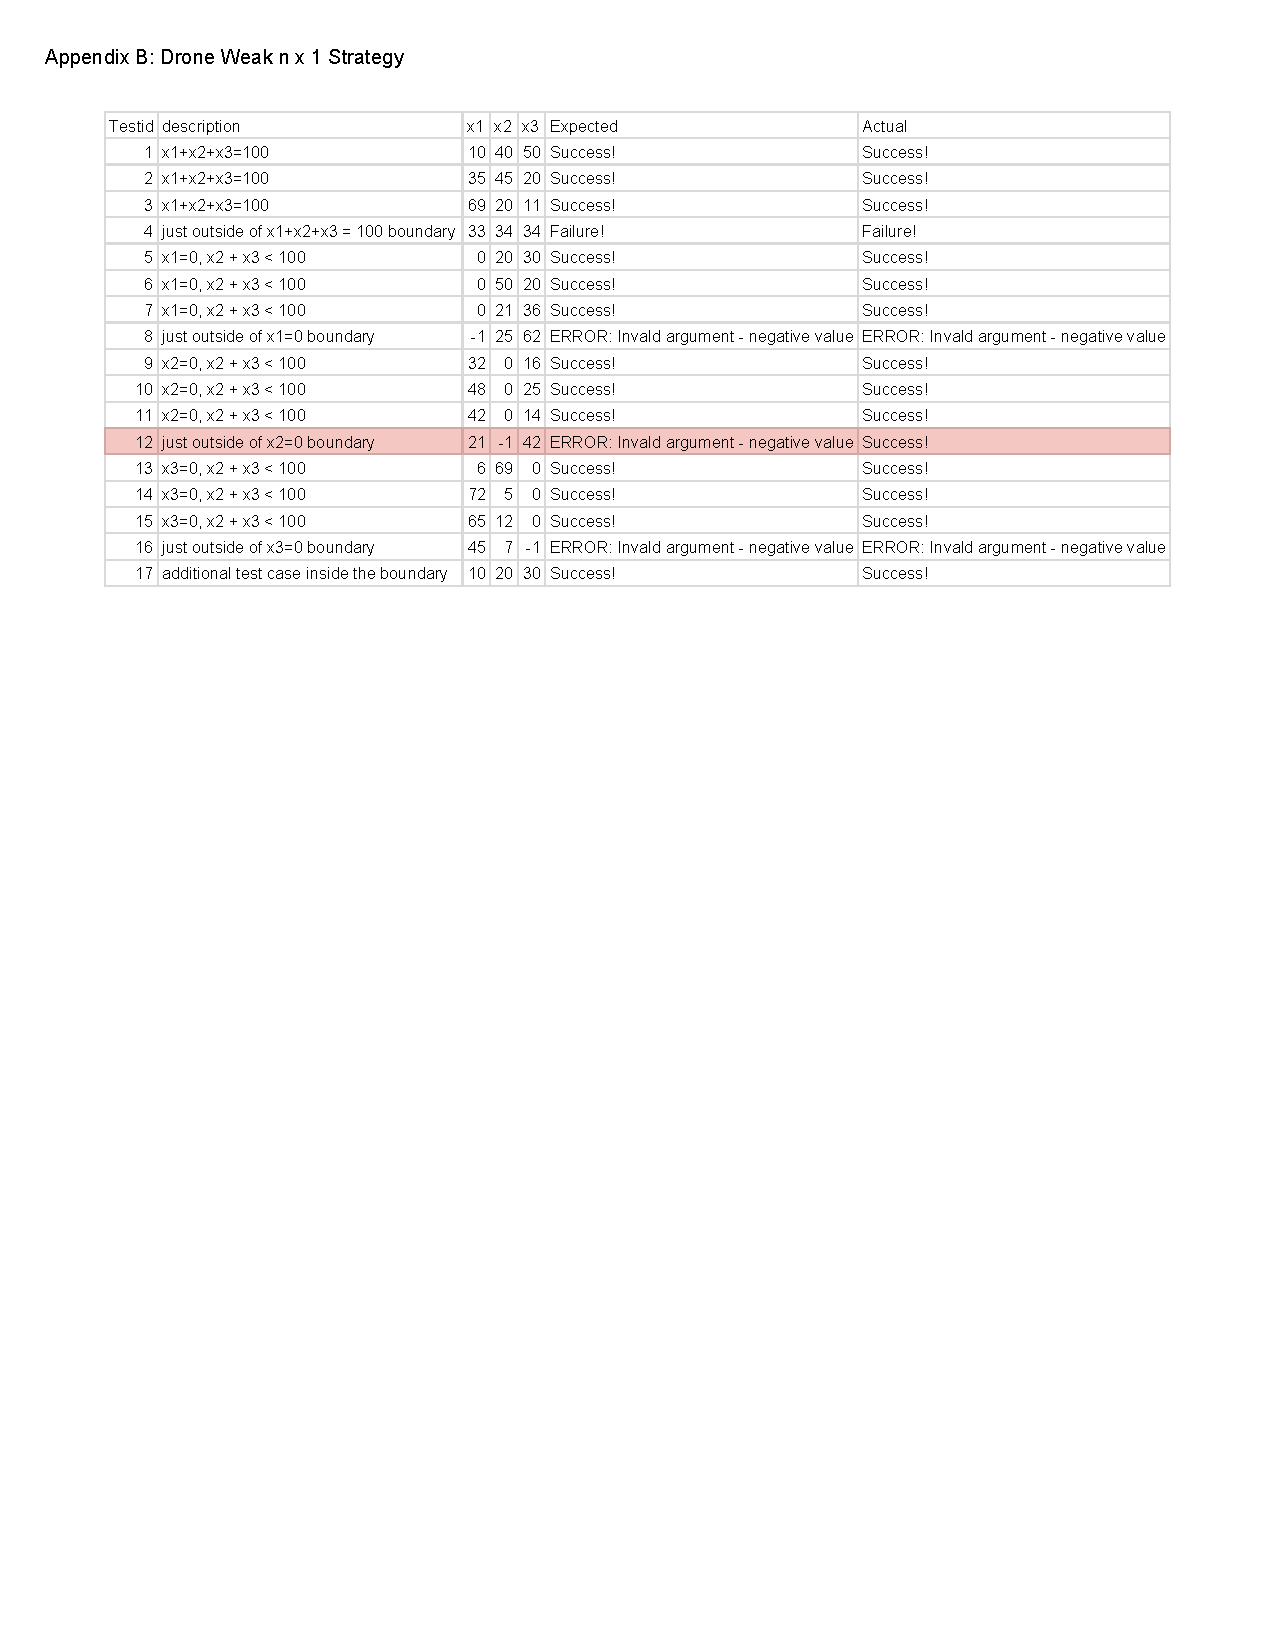
\includepdf[]{weaknx1-drone-table.pdf}

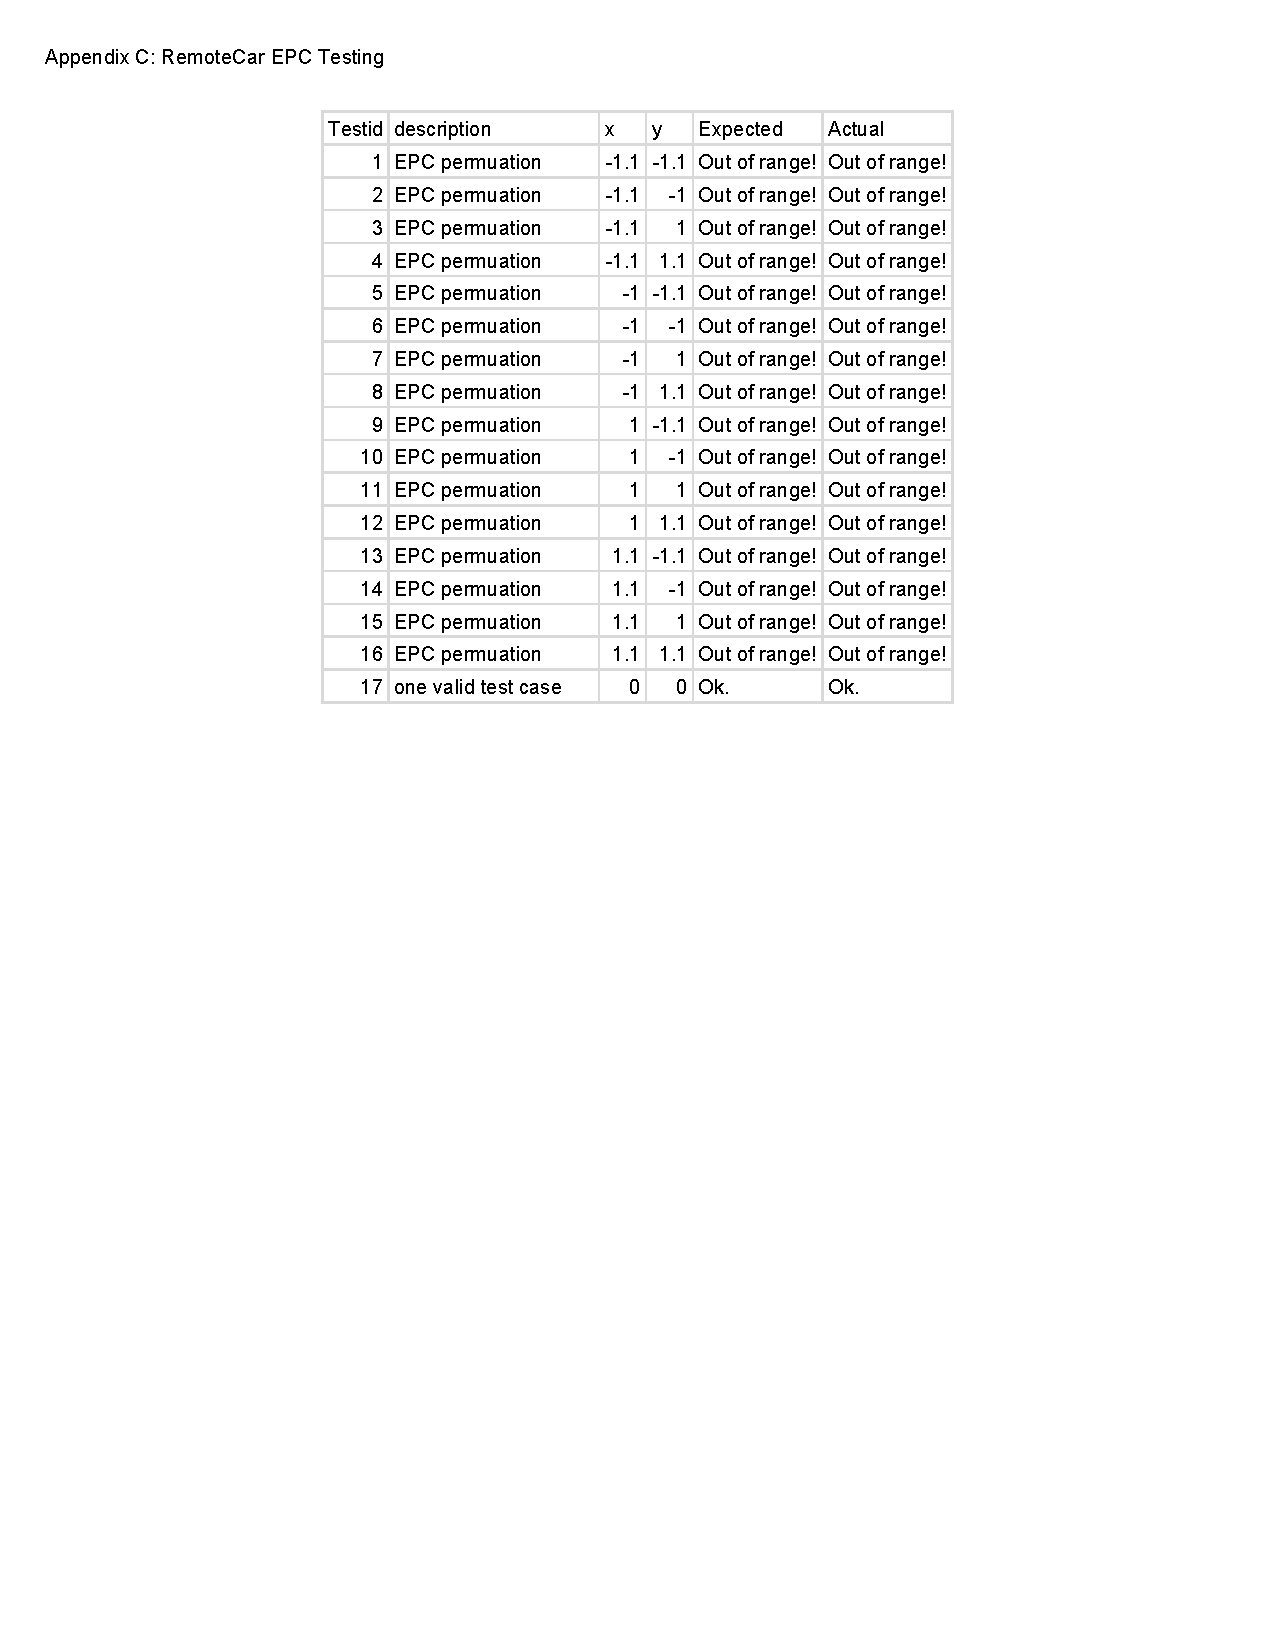
\includepdf[]{EPC-remotecar-table.pdf}
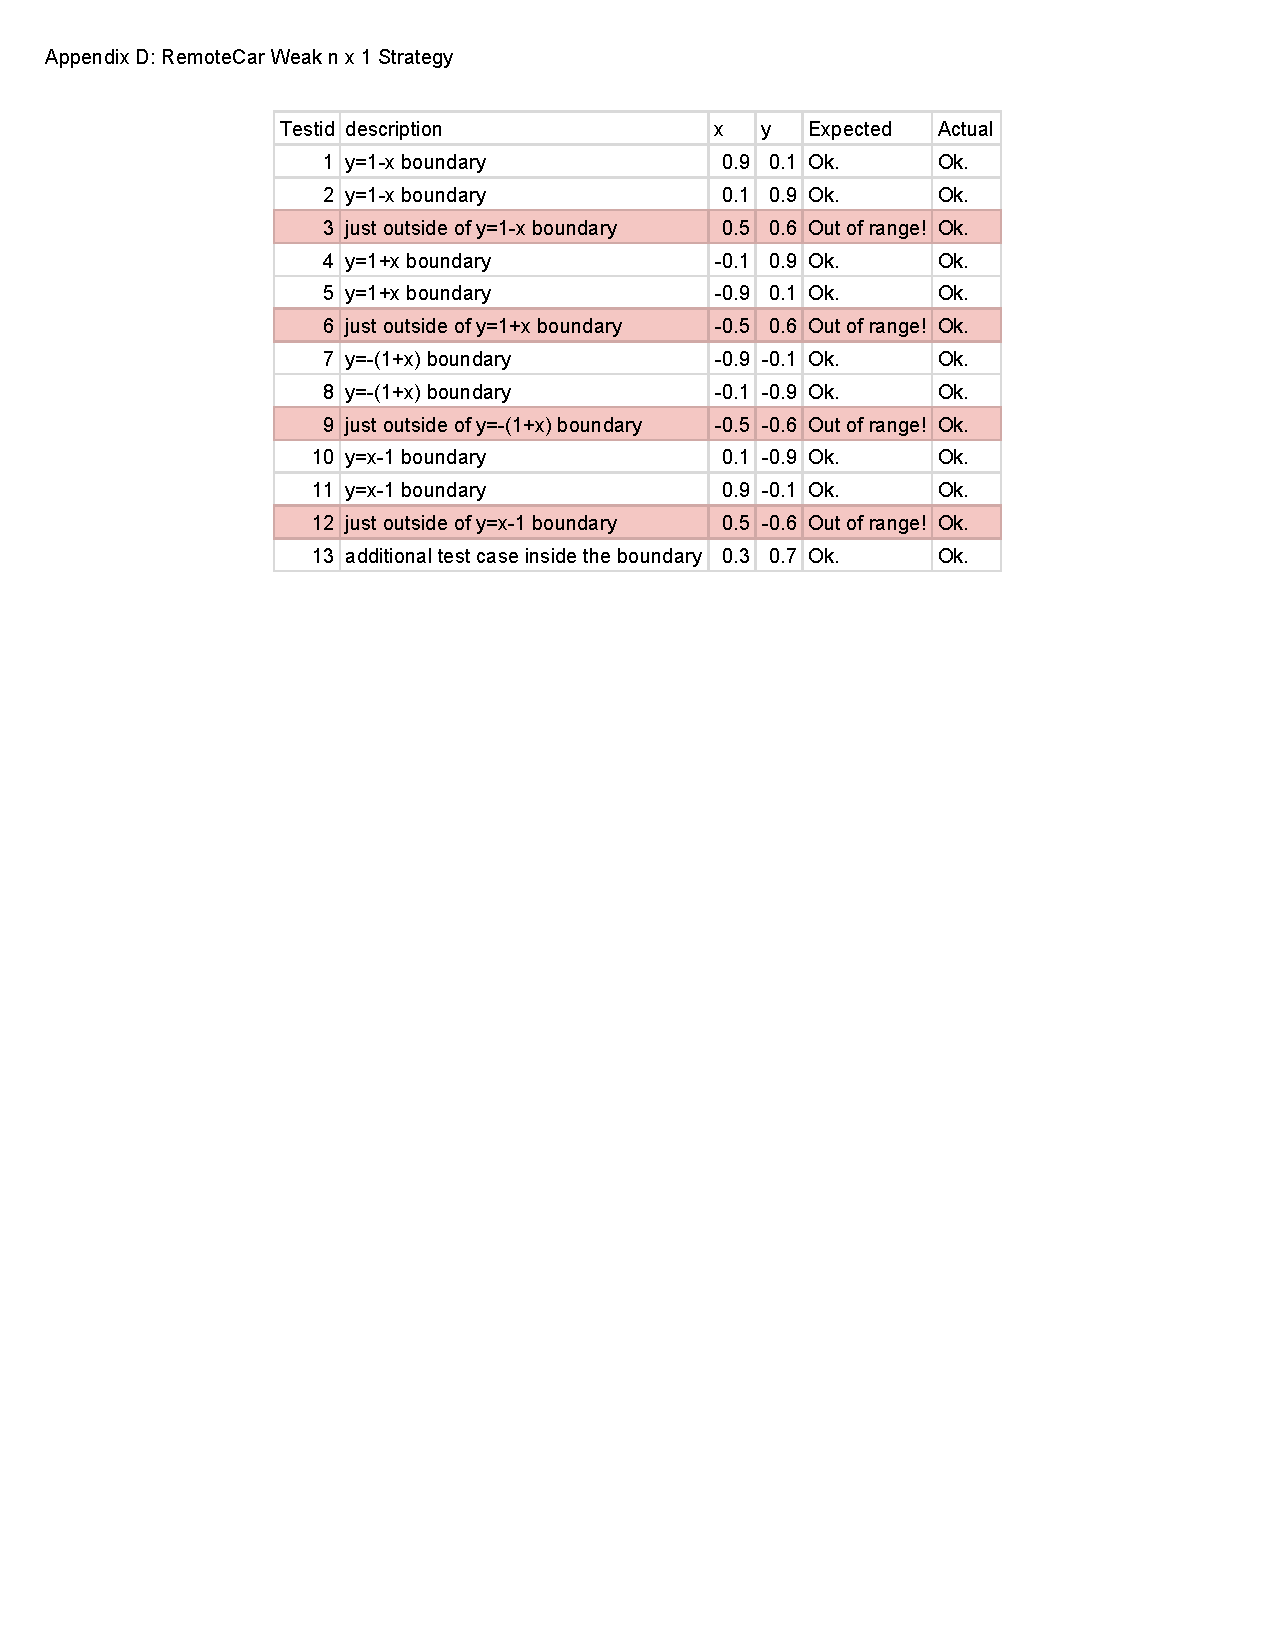
\includepdf[]{weaknx1-remotecar-table.pdf}

\end{document}
